\documentclass[UTF8]{ctexart}
\usepackage[a4paper,margin=1.8cm]{geometry}
\usepackage{graphicx}
\usepackage{float}
\usepackage{longtable}
\usepackage{array}
\usepackage{xcolor}
\usepackage{fancyvrb}
\usepackage{hyperref}
\setlength{\parindent}{0pt}
\setlength{\parskip}{0.45em}
\begin{document}
\section*{代码生成与寄存器分配完整模拟卷 05（题目与完整解析）}

\subsection*{卷面说明}

\begin{Verbatim}[fontsize=\small,breaklines=true]
考试时间：120 分钟
总分：100 分
说明：本卷独立覆盖指令选择、指令代价、基本块/流图、活跃性、DAG 优化、描述符和 getReg。
目标机语义及代价均在题面中给出。
\end{Verbatim}

\subsection*{A 卷题目}

\subsubsection*{一、指令选择与目标代码代价（20 分）}

目标机有寄存器 \texttt{R0、R1}，指令及代价如下：

\begin{Verbatim}[fontsize=\small,breaklines=true]
LD   R, x       ; R=x                 代价 2
ST   x, R       ; x=R                 代价 2
ADD  Rd, Rs     ; Rd=Rd+Rs            代价 1
ADDI R, k       ; R=R+k               代价 1
INC  x          ; x=x+1               代价 1
\end{Verbatim}

1. 为三地址语句 \texttt{x=y+z} 生成目标代码并计算总代价。 2. 用通用 \texttt{LD/ADDI/ST} 序列实现 \texttt{a=a+1}，计算代价。 3. 再用 \texttt{INC a} 实现同一语句，计算节省的代价。 4. 说明同一 IR 为什么可能对应多个目标指令序列。 5. 写出代码生成器在指令选择时必须考虑的三个因素。

\subsubsection*{二、基本块划分、流图与循环（20 分）}

给定三地址指令：

\begin{Verbatim}[fontsize=\small,breaklines=true]
(1)  b = 1
(2)  n = 10
(3)  d = l + n
(4)  c = 2
(5)  t1 = 4 * a
(6)  t2 = l + n
(7)  c = c + b
(8)  if c < n goto (6)
(9)  a = a + b
(10) if a < n goto (4)
(11) c = a - b
\end{Verbatim}

1. 写出首指令判定规则。 2. 列出全部首指令。 3. 划分基本块。 4. 写出完整 CFG 边集合。 5. 写出回边及对应自然循环。

\subsubsection*{三、活跃性与下一次使用（20 分）}

基本块：

\begin{Verbatim}[fontsize=\small,breaklines=true]
(1) t1 = a - b
(2) t2 = t1 + c
(3) t3 = t2 + d
(4) a  = t3
\end{Verbatim}

块出口处：

\begin{Verbatim}[fontsize=\small,breaklines=true]
LiveOut={a,b,c,d}
t1、t2、t3 不活跃且无后续使用
\end{Verbatim}

1. 写出对语句 \texttt{x=y op z} 反向扫描的更新规则。 2. 计算每条语句之前的活跃变量集合。 3. 写出每个源操作数在块内的下一次使用位置。 4. 指出每条语句的结果在何时变为不活跃。 5. 说明这些信息怎样帮助 \texttt{getReg} 选择可覆盖寄存器。

\subsubsection*{四、基本块 DAG、数组写入与死代码（20 分）}

给定基本块：

\begin{Verbatim}[fontsize=\small,breaklines=true]
(1) x = a[i]
(2) y = a[i]
(3) a[j] = t
(4) z = a[i]
(5) u = b + 1
(6) v = b + 1
(7) w = v * 1
\end{Verbatim}

已知无法证明 \texttt{i!=j}，块出口活跃变量为：

\begin{Verbatim}[fontsize=\small,breaklines=true]
LiveOut={x,z,u}
\end{Verbatim}

1. 指出可以合并的公共子表达式。 2. 说明数组写入 \texttt{(3)} 为什么会杀死此前的 \texttt{a[i]} 结果。 3. 对 \texttt{(7)} 做代数化简。 4. 删除死代码后写出最终基本块。 5. 区分死代码和不可达代码。

\subsubsection*{五、描述符、getReg 与两寄存器代码生成（20 分）}

目标机只有 \texttt{R0、R1}，采用两地址指令：

\begin{Verbatim}[fontsize=\small,breaklines=true]
LD  R, x       ; R=x
ST  x, R       ; x=R
ADD Rd, Rs     ; Rd=Rd+Rs
SUB Rd, Rs     ; Rd=Rd-Rs
\end{Verbatim}

三地址码：

\begin{Verbatim}[fontsize=\small,breaklines=true]
t1 = a - b
t2 = a - c
t3 = t1 + t2
d  = t3 + t2
\end{Verbatim}

1. 写出寄存器描述符和地址描述符的定义。 2. 给出一组完整目标代码，允许把临时变量溢出到内存。 3. 逐条写出 \texttt{R0、R1} 中保存的值。 4. 指出哪一步发生 spill，哪一步发生 reload。 5. 写出结束时 \texttt{d} 的地址描述符。

\subsection*{B 按考试标准重写答案}

\subsubsection*{一、指令选择与目标代码代价答案}

\paragraph*{1. `x=y+z`}

目标机是寄存器-寄存器加法，因此先把两个操作数装入寄存器，再相加并写回：

\begin{Verbatim}[fontsize=\small,breaklines=true]
LD  R0, y      ; 代价 2
LD  R1, z      ; 代价 2
ADD R0, R1     ; 代价 1，R0=y+z
ST  x, R0      ; 代价 2
\end{Verbatim}

总代价：

\begin{Verbatim}[fontsize=\small,breaklines=true]
2 + 2 + 1 + 2 = 7
\end{Verbatim}

\paragraph*{2. 用通用序列实现 `a=a+1`}

\begin{Verbatim}[fontsize=\small,breaklines=true]
LD   R0, a     ; 代价 2
ADDI R0, 1     ; 代价 1
ST   a, R0     ; 代价 2
\end{Verbatim}

总代价：

\begin{Verbatim}[fontsize=\small,breaklines=true]
2 + 1 + 2 = 5
\end{Verbatim}

\paragraph*{3. 用 `INC a`}

\begin{Verbatim}[fontsize=\small,breaklines=true]
INC a          ; 代价 1
\end{Verbatim}

节省代价：

\begin{Verbatim}[fontsize=\small,breaklines=true]
5 - 1 = 4
\end{Verbatim}

\paragraph*{4. 同一 IR 对应多个目标序列的原因}

同一条 IR 只描述语义，不指定机器指令形态。目标机可能有多种实现方式：

\begin{longtable}{|p{0.47\linewidth}|p{0.47\linewidth}|}
\hline
IR 语义 & 实现方式 \\
\hline
\endfirsthead
IR 语义 & 实现方式 \\
\hline
\endhead
\texttt{a=a+1} & \texttt{LD/ADDI/ST} \\
\hline
\texttt{a=a+1} & \texttt{INC a} \\
\hline
\texttt{x=y+z} & 不同寄存器分配、不同装载顺序 \\
\hline
\end{longtable}

只要最终可观察结果一致，代码生成器可以选择不同寻址方式、寄存器和专用指令。

\paragraph*{5. 指令选择考虑因素}

\begin{longtable}{|p{0.47\linewidth}|p{0.47\linewidth}|}
\hline
因素 & 说明 \\
\hline
\endfirsthead
因素 & 说明 \\
\hline
\endhead
目标 ISA & 指令语义、寻址方式、是否有立即数或复合指令 \\
\hline
代码代价 & 指令条数、执行周期、访存次数 \\
\hline
寄存器压力 & 当前可用寄存器数量，是否会造成 spill \\
\hline
IR 信息 & IR 是否保留类型、内存访问、常量等信息 \\
\hline
后续优化 & 是否便于调度、寄存器分配和流水线执行 \\
\hline
\end{longtable}

\subsubsection*{二、基本块划分、流图与循环答案}

\paragraph*{1. 首指令判定规则}

首指令有三类：

\begin{Verbatim}[fontsize=\small,breaklines=true]
1. 整个程序或指令序列的第一条指令。
2. 任意跳转指令的目标指令。
3. 紧跟在跳转指令之后的指令。
\end{Verbatim}

\paragraph*{2. 全部首指令}

\begin{longtable}{|p{0.47\linewidth}|p{0.47\linewidth}|}
\hline
首指令 & 原因 \\
\hline
\endfirsthead
首指令 & 原因 \\
\hline
\endhead
(1) & 第一条指令 \\
\hline
(4) & 指令 (10) 的跳转目标 \\
\hline
(6) & 指令 (8) 的跳转目标 \\
\hline
(9) & 紧跟在条件跳转 (8) 后 \\
\hline
(11) & 紧跟在条件跳转 (10) 后 \\
\hline
\end{longtable}

\paragraph*{3. 基本块划分}

\begin{longtable}{|p{0.47\linewidth}|p{0.47\linewidth}|}
\hline
基本块 & 指令范围 \\
\hline
\endfirsthead
基本块 & 指令范围 \\
\hline
\endhead
B1 & (1)-(3) \\
\hline
B2 & (4)-(5) \\
\hline
B3 & (6)-(8) \\
\hline
B4 & (9)-(10) \\
\hline
B5 & (11) \\
\hline
\end{longtable}

\paragraph*{4. CFG 边集合}

\begin{figure}[H]\centering
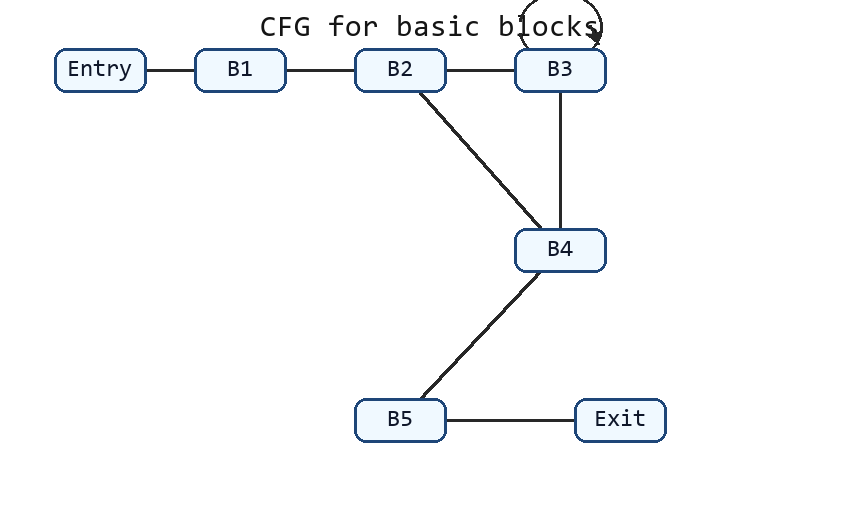
\includegraphics[width=0.82\linewidth]{figures/cfg-09-basic-blocks.png}
\par{\small 基本块 CFG}
\end{figure}

\begin{longtable}{|p{0.47\linewidth}|p{0.47\linewidth}|}
\hline
边 & 原因 \\
\hline
\endfirsthead
边 & 原因 \\
\hline
\endhead
B1 -> B2 & B1 顺序落到 B2 \\
\hline
B2 -> B3 & B2 顺序落到 B3 \\
\hline
B3 -> B3 & (8) 条件为真，跳到 (6) \\
\hline
B3 -> B4 & (8) 条件为假，顺序到 (9) \\
\hline
B4 -> B2 & (10) 条件为真，跳到 (4) \\
\hline
B4 -> B5 & (10) 条件为假，顺序到 (11) \\
\hline
B5 -> Exit & 程序片段结束 \\
\hline
\end{longtable}

\paragraph*{5. 回边和自然循环}

回边定义：边 \texttt{n -> h} 中，若 \texttt{h} 支配 \texttt{n}，则该边为回边。

\begin{longtable}{|p{0.31\linewidth}|p{0.31\linewidth}|p{0.31\linewidth}|}
\hline
回边 & 判断 & 自然循环 \\
\hline
\endfirsthead
回边 & 判断 & 自然循环 \\
\hline
\endhead
B3 -> B3 & 自身支配自身 & \texttt{\textbackslash{}\{B3\textbackslash{}\}} \\
\hline
B4 -> B2 & B2 支配 B4 & \texttt{\textbackslash{}\{B2,B3,B4\textbackslash{}\}} \\
\hline
\end{longtable}

B4 到 B2 的自然循环从回边尾 B4 反向找前驱，直到回边头 B2，得到 B4、B3、B2。

\subsubsection*{三、活跃性与下一次使用答案}

\paragraph*{1. 反向扫描规则}

对语句：

\begin{Verbatim}[fontsize=\small,breaklines=true]
x = y op z
\end{Verbatim}

从基本块末尾向前扫描：

\begin{Verbatim}[fontsize=\small,breaklines=true]
1. 先记录该语句处 x、y、z 当前的 live 和 next-use 信息。
2. 因为本语句重新定义 x，所以把 x 设为不活跃，next-use 设为空。
3. 因为本语句使用 y、z，所以把 y、z 设为活跃，next-use 设为当前语句编号。
\end{Verbatim}

\paragraph*{2. 每条语句之前的活跃变量集合}

出口：

\begin{Verbatim}[fontsize=\small,breaklines=true]
LiveOut = {a,b,c,d}
\end{Verbatim}

反向计算：

\begin{longtable}{|p{0.47\linewidth}|p{0.47\linewidth}|}
\hline
位置 & 活跃变量 \\
\hline
\endfirsthead
位置 & 活跃变量 \\
\hline
\endhead
语句 (4) 之后 & \texttt{\textbackslash{}\{a,b,c,d\textbackslash{}\}} \\
\hline
语句 (4) 之前 & \texttt{\textbackslash{}\{b,c,d,t3\textbackslash{}\}} \\
\hline
语句 (3) 之前 & \texttt{\textbackslash{}\{b,c,d,t2\textbackslash{}\}} \\
\hline
语句 (2) 之前 & \texttt{\textbackslash{}\{b,c,d,t1\textbackslash{}\}} \\
\hline
语句 (1) 之前 & \texttt{\textbackslash{}\{a,b,c,d\textbackslash{}\}} \\
\hline
\end{longtable}

以语句 (4) 为例：

\begin{Verbatim}[fontsize=\small,breaklines=true]
a = t3
before = (after - {a}) union {t3}
       = {b,c,d,t3}
\end{Verbatim}

\paragraph*{3. 源操作数下一次使用}

\begin{longtable}{|p{0.31\linewidth}|p{0.31\linewidth}|p{0.31\linewidth}|}
\hline
位置 & 源操作数 & 下一次使用 \\
\hline
\endfirsthead
位置 & 源操作数 & 下一次使用 \\
\hline
\endhead
语句 (1) 前 & a, b & (1) \\
\hline
语句 (2) 前 & t1, c & (2) \\
\hline
语句 (3) 前 & t2, d & (3) \\
\hline
语句 (4) 前 & t3 & (4) \\
\hline
\end{longtable}

\paragraph*{4. 结果何时变为不活跃}

\begin{longtable}{|p{0.23\linewidth}|p{0.23\linewidth}|p{0.23\linewidth}|p{0.23\linewidth}|}
\hline
结果 & 产生位置 & 最后一次使用 & 之后状态 \\
\hline
\endfirsthead
结果 & 产生位置 & 最后一次使用 & 之后状态 \\
\hline
\endhead
t1 & (1) & (2) & 语句 (2) 后不活跃 \\
\hline
t2 & (2) & (3) & 语句 (3) 后不活跃 \\
\hline
t3 & (3) & (4) & 语句 (4) 后不活跃 \\
\hline
新 a & (4) & 块外仍活跃 & 出口活跃 \\
\hline
\end{longtable}

\paragraph*{5. 对 getReg 的帮助}

\texttt{getReg} 选择寄存器时优先覆盖“后面不再使用”的值：

\begin{longtable}{|p{0.47\linewidth}|p{0.47\linewidth}|}
\hline
情况 & 策略 \\
\hline
\endfirsthead
情况 & 策略 \\
\hline
\endhead
某寄存器中的值之后不活跃 & 可直接覆盖 \\
\hline
值之后活跃但内存已有最新副本 & 可覆盖寄存器副本 \\
\hline
所有值都活跃且无内存副本 & 选择下一次使用最晚的值 spill \\
\hline
\end{longtable}

因此活跃性和下一次使用信息能减少不必要的 \texttt{ST} 和 \texttt{LD}。

\subsubsection*{四、基本块 DAG、数组写入与死代码答案}

\paragraph*{1. 可合并的公共子表达式}

\begin{longtable}{|p{0.31\linewidth}|p{0.31\linewidth}|p{0.31\linewidth}|}
\hline
表达式 & 可否合并 & 原因 \\
\hline
\endfirsthead
表达式 & 可否合并 & 原因 \\
\hline
\endhead
(1) \texttt{a[i]} 与 (2) \texttt{a[i]} & 可以 & 两者之间没有写 \texttt{a}，也没有修改 \texttt{i} \\
\hline
(5) \texttt{b+1} 与 (6) \texttt{b+1} & 可以 & 两者操作数相同，且 \texttt{b} 未变 \\
\hline
(1)/(2) \texttt{a[i]} 与 (4) \texttt{a[i]} & 不可以 & 中间有 (3) \texttt{a[j]=t} \\
\hline
\end{longtable}

\paragraph*{2. 数组写入为什么 kill 先前读取}

题目明确无法证明 \texttt{i != j}。因此 \texttt{a[j]=t} 可能写的就是 \texttt{a[i]}：

\begin{Verbatim}[fontsize=\small,breaklines=true]
若 i == j，则 a[j] 与 a[i] 是同一位置。
\end{Verbatim}

所以 (3) 必须杀死此前关于数组 \texttt{a} 的读取结果，(4) 的 \texttt{z=a[i]} 需要重新读取。

\paragraph*{3. 代数化简}

\begin{Verbatim}[fontsize=\small,breaklines=true]
w = v * 1
\end{Verbatim}

可化简为：

\begin{Verbatim}[fontsize=\small,breaklines=true]
w = v
\end{Verbatim}

\paragraph*{4. 删除死代码后的最终基本块}

出口活跃变量为：

\begin{Verbatim}[fontsize=\small,breaklines=true]
LiveOut = {x,z,u}
\end{Verbatim}

\texttt{y}、\texttt{v}、\texttt{w} 在出口不活跃，且它们的值不影响活跃变量。因此最终保留：

\begin{Verbatim}[fontsize=\small,breaklines=true]
(1) x = a[i]
(3) a[j] = t
(4) z = a[i]
(5) u = b + 1
\end{Verbatim}

说明：\texttt{a[j]=t} 即使没有变量名出现在 LiveOut 中也不能删，因为数组写入是内存副作用。

\paragraph*{5. 死代码与不可达代码}

\begin{longtable}{|p{0.47\linewidth}|p{0.47\linewidth}|}
\hline
类型 & 含义 \\
\hline
\endfirsthead
类型 & 含义 \\
\hline
\endhead
死代码 & 会被执行，但计算结果以后不再使用，且删除不改变可观察行为 \\
\hline
不可达代码 & 从 CFG 入口没有路径到达，运行时不会执行 \\
\hline
\end{longtable}

\subsubsection*{五、描述符、getReg 与两寄存器代码生成答案}

\paragraph*{1. 描述符定义}

\begin{longtable}{|p{0.47\linewidth}|p{0.47\linewidth}|}
\hline
描述符 & 定义 \\
\hline
\endfirsthead
描述符 & 定义 \\
\hline
\endhead
寄存器描述符 \texttt{RegDesc(R)} & 记录寄存器 R 当前保存哪些变量或临时变量的最新值 \\
\hline
地址描述符 \texttt{AddrDesc(x)} & 记录变量 x 的最新值当前在哪些位置：内存、寄存器或两者都有 \\
\hline
\end{longtable}

\paragraph*{2. 一组完整目标代码}

只有两个寄存器，计算 \texttt{t2} 时需要覆盖保存 \texttt{t1} 的寄存器，所以先 spill \texttt{t1} 到内存，后面再 reload。

\begin{Verbatim}[fontsize=\small,breaklines=true]
LD  R0, a
LD  R1, b
SUB R0, R1      ; R0 = t1
ST  t1, R0      ; spill t1

LD  R0, a
LD  R1, c
SUB R0, R1      ; R0 = t2

LD  R1, t1      ; reload t1
ADD R1, R0      ; R1 = t3 = t1 + t2
ADD R1, R0      ; R1 = d  = t3 + t2
ST  d, R1
\end{Verbatim}

\paragraph*{3. 寄存器内容变化}

\begin{longtable}{|p{0.23\linewidth}|p{0.23\linewidth}|p{0.23\linewidth}|p{0.23\linewidth}|}
\hline
步骤 & 指令 & R0 & R1 \\
\hline
\endfirsthead
步骤 & 指令 & R0 & R1 \\
\hline
\endhead
初始 & - & \texttt{\textbackslash{}\{\textbackslash{}\}} & \texttt{\textbackslash{}\{\textbackslash{}\}} \\
\hline
1 & \texttt{LD R0,a} & \texttt{\textbackslash{}\{a\textbackslash{}\}} & \texttt{\textbackslash{}\{\textbackslash{}\}} \\
\hline
2 & \texttt{LD R1,b} & \texttt{\textbackslash{}\{a\textbackslash{}\}} & \texttt{\textbackslash{}\{b\textbackslash{}\}} \\
\hline
3 & \texttt{SUB R0,R1} & \texttt{\textbackslash{}\{t1\textbackslash{}\}} & \texttt{\textbackslash{}\{b\textbackslash{}\}} \\
\hline
4 & \texttt{ST t1,R0} & \texttt{\textbackslash{}\{t1\textbackslash{}\}} & \texttt{\textbackslash{}\{b\textbackslash{}\}} \\
\hline
5 & \texttt{LD R0,a} & \texttt{\textbackslash{}\{a\textbackslash{}\}} & \texttt{\textbackslash{}\{b\textbackslash{}\}} \\
\hline
6 & \texttt{LD R1,c} & \texttt{\textbackslash{}\{a\textbackslash{}\}} & \texttt{\textbackslash{}\{c\textbackslash{}\}} \\
\hline
7 & \texttt{SUB R0,R1} & \texttt{\textbackslash{}\{t2\textbackslash{}\}} & \texttt{\textbackslash{}\{c\textbackslash{}\}} \\
\hline
8 & \texttt{LD R1,t1} & \texttt{\textbackslash{}\{t2\textbackslash{}\}} & \texttt{\textbackslash{}\{t1\textbackslash{}\}} \\
\hline
9 & \texttt{ADD R1,R0} & \texttt{\textbackslash{}\{t2\textbackslash{}\}} & \texttt{\textbackslash{}\{t3\textbackslash{}\}} \\
\hline
10 & \texttt{ADD R1,R0} & \texttt{\textbackslash{}\{t2\textbackslash{}\}} & \texttt{\textbackslash{}\{d\textbackslash{}\}} \\
\hline
11 & \texttt{ST d,R1} & \texttt{\textbackslash{}\{t2\textbackslash{}\}} & \texttt{\textbackslash{}\{d\textbackslash{}\}} \\
\hline
\end{longtable}

\paragraph*{4. spill 和 reload}

\begin{longtable}{|p{0.31\linewidth}|p{0.31\linewidth}|p{0.31\linewidth}|}
\hline
类型 & 指令 & 原因 \\
\hline
\endfirsthead
类型 & 指令 & 原因 \\
\hline
\endhead
spill & \texttt{ST t1,R0} & 后面还要用 t1，但 R0 要被重新用于计算 t2 \\
\hline
reload & \texttt{LD R1,t1} & 计算 t3 时需要重新取回 t1 \\
\hline
\end{longtable}

\paragraph*{5. 结束时 `d` 的地址描述符}

最后执行了：

\begin{Verbatim}[fontsize=\small,breaklines=true]
ST d, R1
\end{Verbatim}

因此 \texttt{d} 的最新值既在 R1，也在内存 d 中：

\begin{Verbatim}[fontsize=\small,breaklines=true]
AddrDesc(d) = {R1, 内存位置 d}
\end{Verbatim}
\end{document}
